\section{介绍}

《星际拓荒》（\emph{Outer Wilds}）是一款由 Mobius Digital 开发、Annapurna Interactive 发行的开放世界太空探索游戏。它的表层形式并不复杂：玩家扮演一名刚刚取得飞行资格的新手宇航员，驾驶一艘小型飞船，在一个微缩太阳系中探索不同星球、遗迹和自然现象。然而，只要真正进入游戏，就会发现它与常见开放世界作品的差异非常明显。游戏几乎不提供传统意义上的任务清单，没有等级、装备、技能树，也没有以战斗为核心的成长路线。玩家面对的不是一张布满图标的地图，而是一个正在自行运转的宇宙。

\begin{figure}[H]
    \centering
    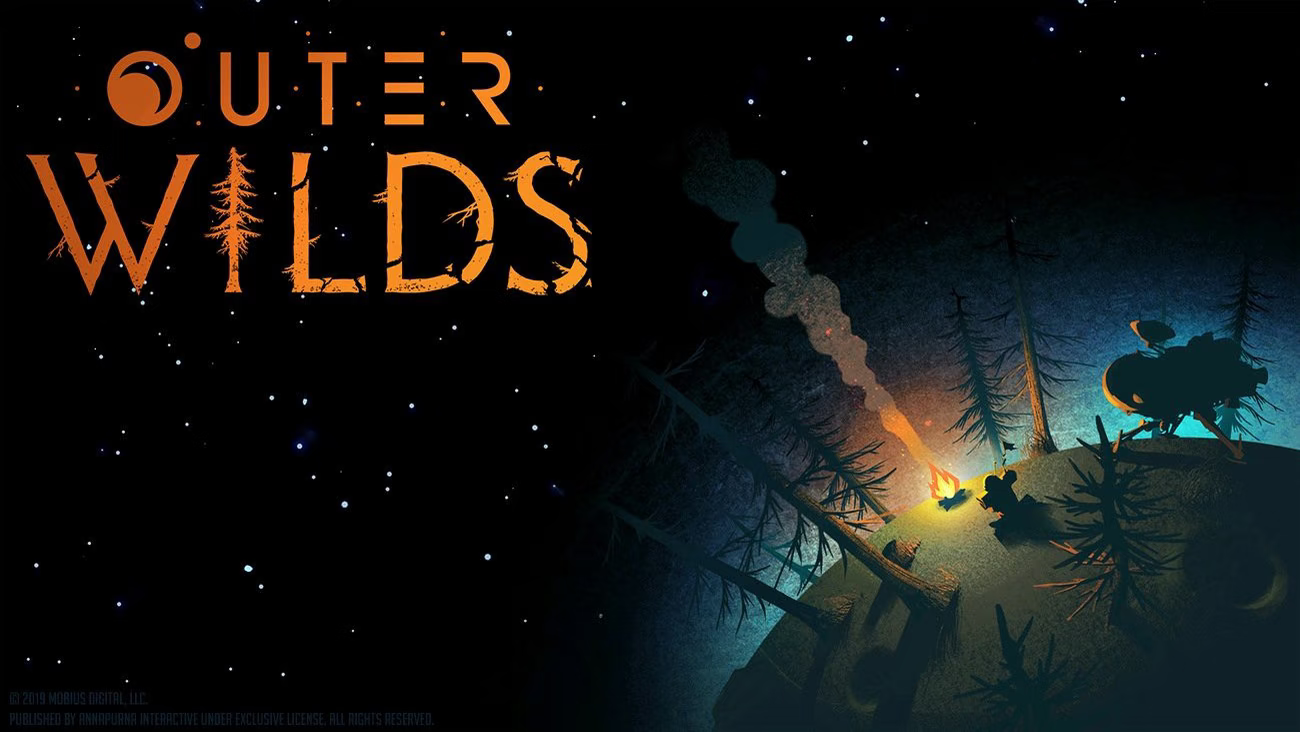
\includegraphics[width=0.8\textwidth]{Img/intro.jpg}
    \caption{星际拓荒游戏封面}
\end{figure}

这种设计很容易在初见时造成疑惑：如果没有明确任务，没有数值奖励，也没有角色能力提升，玩家为什么还要继续探索？《星际拓荒》的回答是好奇心。远处星球上无法解释的爆炸，博物馆里暗示未知文明的展品，来自不同方向的信号，随时间变化的天体环境，都在不断向玩家提出问题。游戏并不急着告诉玩家“应该做什么”，而是让玩家自己意识到“我想知道那里发生了什么”。这使它的探索动力与许多依靠任务驱动、战斗反馈或资源收集的作品不同：玩家真正追逐的不是外部奖励，而是对世界的理解。

本文将从游戏设计角度分析《星际拓荒》的核心体验：它如何把知识设计成奖励，如何用隐性引导组织看似自由的探索，如何利用时间循环和科学规则形成信息锁，又如何通过碎片化叙事让玩家主动拼合世界。最后我会简单讲一下这个游戏的十分优秀的音乐。由于《星际拓荒》的关键体验高度依赖第一次发现，本文会尽量避免揭露终极谜题和结局细节，只讨论设计结构与体验机制。

